\section{Simulation Testbed}
\label{sec:exp}

This section details our experimental settings in terms of the hardware
parameters, the database and query workload, and the performance metrics
on which we evaluated the PCM-conscious operator implementations.



\subsection{Architectural Platform}
Since PCM memory is as yet not commercially available, we
have taken recourse to a simulated hardware environment to
evaluate the impact of the PCM-conscious operators.  For this
purpose, we chose Multi2sim~\cite{multi2sim}, an open-source
application-only\footnote{Simulates only the application layer without
the OS stack.} simulator.

\begin{center}
\begin{table}[h]
\begin{small}
\caption{Experimental Setup}
\label{table:setup}
\begin{tabular}{p{4cm}p{12cm}}
\toprule
Simulator & Multi2sim-4.2 with added support for PCM\\ \hline

L1D cache (private) & 32KB, 64B line, 4-way set-associative, 4 cycle latency, write-back, LRU\\ \hline
L1I cache (private) & 32KB, 64B line, 4-way set-associative, 4 cycle latency, write-back, LRU\\ \hline   
L2 cache (private) & 256KB, 64B line, 4-way set-associative, 11 cycle latency, write-back, LRU\\ \hline

DRAM buffer (private) & 4MB, 256B line, 8-way set-associative, 200 cycle latency, write-back, N-Chance (N = 4)\\ \hline

Main Memory & 2GB PCM, 4KB page, 1024 cycle read latency (per 256B line), 64 cycle write latency (per 4B modified word)\\ \bottomrule
\end{tabular}
\end{small}
\end{table}
\end{center}

We evaluated the algorithms on Multi2sim in cycle-accurate simulation
mode. Since it does not have native support for PCM, we made a major
extension to its existing memory module to model PCM memory. Specifically,
the following enhancements were incorporated in the simulator to conduct
our experimental evaluation:

\textbf{Hybrid Main Memory}: 
The memory organization was extended such that the new configuration
consists of PCM with a hardware controlled DRAM buffer. The DRAM buffer
acts as another level of cache in the memory hierarchy, specifically
between the L2 cache and the PCM.

\textbf{New DRAM Replacement Policy}: 
The DRAM is simulated as a set-associative write-back memory with
\textit{N-Chance} as the eviction policy. As mentioned in \cite{nchance},
$N$ was set to $\frac{K}{2}$, where $K$ is the cache associativity,
since this setting was found to provide good performance on multiple
metrics -- writes, energy and latency.

\textbf{Tracking DRAM-PCM Data}:
Like most other architectural simulators, Multi2sim does not explicitly
track the data residing at the different levels of the memory
hierarchy. It instead maintains only a single buffer that indicates
the latest data, as visible to the simulated program, for each memory
location. We therefore had to add separate data tracking functionality
for the DRAM and PCM resident data.

\textbf{Data Comparison Write Scheme}: 
The write-back mechanism of data from DRAM to PCM was modelled on the
DCW~\cite{write} scheme. Thus, for each evicted DRAM block, a comparison
to the original PCM resident data block was made, and writes were
restricted to only those words where the data bits differed. In our
experiments, we measured writes at \textit{word} (4B) granularity.

\textbf{Asymmetric Read-Write Latencies}:  
The timing simulation was modified to account for the higher write
latency of PCM as compared to a read.

\textbf{Wear Distribution}: 
Apart from the raw number of writes, a critical related metric for PCM
algorithms is their wear distribution. We therefore instrumented the
Multi2sim code to track block level wear distribution information. To
achieve this, separate counters were created that tracked writes to each
PCM \textit{line} (256B) during the query processing activity.

\textbf{Intermediate Statistics}: 
Multi2sim does not have support to track intermediate statistics during
a program run. We therefore provided additional inter-process communication capabilities in the
tool so that the simulated program could ask the simulator to dump
statistics for each intermediate operator during the execution of a query.


The specific configurations of the memory hierarchy \emph{(L1 Data,
L1 Instruction, L2, DRAM Buffer, PCM)} used for evaluation in our experiments are
enumerated in Table~\ref{table:setup}.  These values are scaled-down
versions, w.r.t. number of lines, of the hardware simulation parameters used
in \cite{wear} -- the reason for the scaling-down is to ensure that the
simulator running times are not impractically long. However, we have been
careful to ensure that the \emph{ratios} between the capacities of adjacent
levels in the hierarchy are maintained as per the original configurations
in \cite{wear}.  

%\vspace*{0.05in}

\subsection{Database and Queries}
%We used TPC-H (version 2.16.0) 1GB PCM-resident database for our experiments.
For the data, we used the default 1GB database generated by the
TPC-H \cite{tpch} benchmark.  This size is certainly very small compared to the
database sizes typically encountered in modern applications -- however,
we again chose this reduced value to ensure viable simulation running
times. Furthermore, the database is significantly larger than the
simulated DRAM (4MB), representative of most real-world
scenarios.

For simulating our suite of database operators -- \textit{sort},
\textit{hash join} and \textit{group-by} -- we created a separate library
consisting of their native PostgreSQL \cite{postgres} implementations. To
this library, we added the PCM-conscious versions described in the
previous sections.

While we experimented with several of the TPC-H queries, results for
three queries: {\sf Query 13 (Q13)}, {\sf Query 16 (Q16)} and {\sf Query 19 (Q19)}, that
cover a diverse spectrum of the experimental space, are presented here.
For each of the queries, we first identified the execution plan
recommended by the PostgreSQL query optimizer with the native operators,
and then forcibly used the same execution plan for their PCM-conscious
replacements as well. This was done in order to maintain fairness in the
comparison of the PCM-oblivious and PCM-conscious algorithms, though it
is possible that a \emph{better} plan is available for the PCM-conscious
configuration -- we return to this issue 
later in Section~\ref{integration}.  The execution plans associated with the
three queries are shown in Figure~\ref{fig:plan_trees}. 
 


\begin{figure*}[t]
\centering
\subfloat[Q13]{
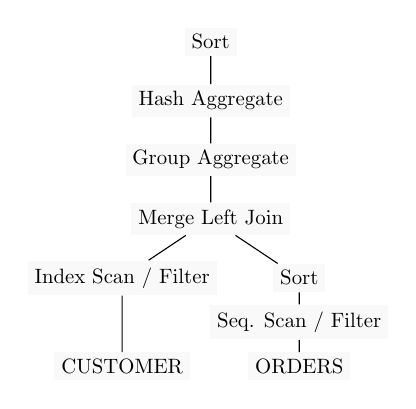
\begin{tikzpicture}[scale=.75, transform shape]

\tikzstyle{every node} = [rectangle, fill=gray!5]

\node (d) at (0,3) {Index Scan / Filter};
\node (c) at (0,1.5) {CUSTOMER};

\node (s) at (3,3) {Sort};
\node (p) at (3,2.25) {Seq. Scan / Filter};
\node (a) at (3,1.5) {ORDERS};

\node (e) at (1.5,4) {Merge Left Join};
\node (f) at (1.5,5)  {Group Aggregate};
\node (g) at (1.5,6)  {Hash Aggregate};
\node (h) at (1.5,7)  {Sort};


\draw[-] (c) -- (d);
\draw[-] (a) -- (p);
\draw[-] (d) -- (e);
\draw[-] (p) -- (s);
\draw[-] (s) -- (e);
\draw[-] (e) -- (f);

\draw[-] (f) -- (g);
\draw[-] (g) -- (h);

\end{tikzpicture}
}
\subfloat[Q16]{
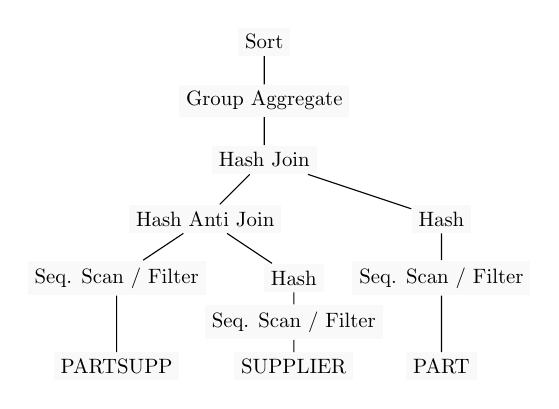
\begin{tikzpicture}[scale=.75, transform shape]

\tikzstyle{every node} = [rectangle, fill=gray!5]

\node (d) at (0,3) {Seq. Scan / Filter};
\node (c) at (0,1.5) {PARTSUPP};

\node (s) at (3,3) {Hash};
\node (p) at (3,2.25) {Seq. Scan / Filter};
\node (a) at (3,1.5) {SUPPLIER};

\node (e) at (1.5,4) {Hash Anti Join};

\node (n) at (5.5, 4) {Hash};
\node (b) at (5.5,3) {Seq. Scan / Filter};
\node (x) at (5.5,1.5) {PART};

\node (f) at (2.5,5)  {Hash Join};
\node (g) at (2.5,6)  {Group Aggregate};
\node (h) at (2.5,7)  {Sort};


\draw[-] (c) -- (d);
\draw[-] (a) -- (p);
\draw[-] (d) -- (e);
\draw[-] (p) -- (s);
\draw[-] (s) -- (e);
\draw[-] (e) -- (f);

\draw[-] (x) -- (b);
\draw[-] (b) -- (n);
\draw[-] (n) -- (f);

\draw[-] (f) -- (g);
\draw[-] (g) -- (h);

\end{tikzpicture}

}
\subfloat[Q19]{


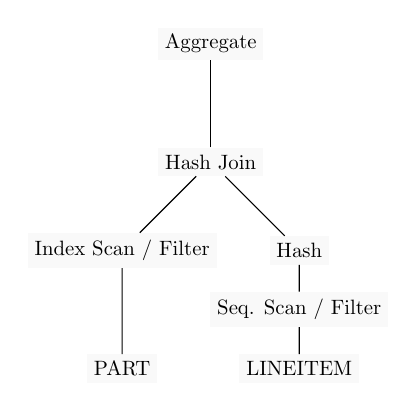
\begin{tikzpicture}[scale=.75, transform shape]

\tikzstyle{every node} = [rectangle, fill=gray!5]

\node (d) at (0,3.5) {Index Scan / Filter};
\node (c) at (0,1.5) {PART};

\node (s) at (3,3.5) {Hash};
\node (p) at (3,2.5) {Seq. Scan / Filter};
\node (a) at (3,1.5) {LINEITEM};

\node (e) at (1.5,5) {Hash Join};
\node (f) at (1.5,7)  {Aggregate};


\draw[-] (c) -- (d);
\draw[-] (a) -- (p);
\draw[-] (d) -- (e);
\draw[-] (p) -- (s);
\draw[-] (s) -- (e);
\draw[-] (e) -- (f);
\end{tikzpicture}
}

\caption{ Query execution plan trees}

\label{fig:plan_trees}

\end{figure*}




\subsection{Performance Metrics}
We measured the following performance metrics for each of the queries:
\begin{description}


\item [PCM Writes:] The total number of word (4B) updates that are applied to the PCM memory during
the query execution.
\item [CPU Cycles:] The total number of CPU cycles required to execute the query.
\item [Wear Distribution:] The frequency distribution of writes measured on a per-256B-block basis.

\end{description}

\section{Experimental Results}
\label{sec:results}
Based on the above framework, we conducted a wide variety of experiments
and present a representative set of results here.  We begin by profiling the
PCM writes and CPU cycles behavior of
the native and PCM-conscious executions for Q13, Q16 and Q19 --
these results are shown in Figure~\ref{fig:overall_results}.  In addition to
the standard TPC-H
with uniform data distribution, we also show results for the sort operator
implementation on a skewed version of TPC-H, generated using a Zipfian distribution
\cite{vivekn} with a skew factor of $Z=1$. In each of these figures,
we provide
both the total and the break-ups on a per-operator basis, with \emph{GB} and
\emph{HJ} labels
denoting group-by and hash join operators, respectively.


\begin{figure*}[htpb]

\centering

\subfloat[Q13 Performance]{
  \includegraphics[height=45mm]{./fig/overall_q13.png}
  
}
%\hspace{0mm}
%\subfloat[Q13 Performance (skewed TPC-H)]{
%  \includegraphics[height=45mm]{./fig/overall_q13_skewed.png}
%  
%}
\hspace{0mm}
\subfloat[Q16 Performance]{
  \includegraphics[height=45mm]{./fig/overall_q16.png}
}
\hspace{0mm}
\subfloat[Q19 Performance]{
  \includegraphics[height=45mm]{./fig/overall_q19.png}
}
\caption{Performance of TPC-H queries}
\label{fig:overall_results}
\end{figure*}


Focusing our attention first on Q13 in
Figure~\ref{fig:overall_results}(a), we find that the bulk of the
overall writes and cycles are consumed by the sort operator. Comparing
the performance of the Native (blue bar) and PCM-conscious (green bar)
implementations, we observe a very significant savings (53\%) on writes,
and an appreciable decrease (20\%) on cycles. For Q13 execution on skewed 
TPC-H, for which we used the multi-pivot flashsort algorithm, 
the corresponding performance numbers (Figure~\ref{fig:overall_results}(b)) are
comparatively lesser. Specifically, savings of 
44\% and 14\%  are observed in writes and cycles, respectively.

Turning our attention to Q16 in Figure~\ref{fig:overall_results}(c),
we find that here it is the group-by operator that primarily influences
the overall writes performance, whereas the hash join determines the
cycles behavior. Again, there are substantial savings in both writes
(40\%) and  cycles (30\%) delivered by the PCM-conscious approach.

Finally, moving on to Q19 in Figure~\ref{fig:overall_results}(d),
where hash join is essentially the only operator, the
savings are around $64\%$ with regard to writes and $32\%$ in cycles.

\subsection{Operator-wise Analysis}
We now analyse the savings due to each operator independently and show
their correspondence to the analyses in Sections~\ref{sort}--\ref{gby} .

\paragraph{Sort.}
For Q13 execution on uniform TPC-H, as already mentioned, we observed 
savings of $53\%$ in writes and $20\%$ in cycles. Similarly, on skewed TPC-H, these  
figures were $44\%$ (writes) and $14\%$ (cycles). 
In the case of Q16, the data at the sorting stage was
found to be much less than the DRAM size. Hence, both the native and
PCM-conscious executions used the standard sort routine, and as a result,
the cycles and writes for both implementations match exactly.

\paragraph{Hash Join.}
Each entry in the hash table consisted of a pointer to the build tuple
and a hash value field. New memory allocation to each bucket was done
in units of pages, with each page holding up to 64 entries. A search for
the matching join column began with the first tuple in the corresponding
bucket, and went on till the last tuple in that bucket, simultaneously
writing out the join tuples for successful matches.  For Q16, we
observed a $12\%$ improvement in writes and $31\%$ in cycles due to the
PCM-conscious hash join, as shown in Figure~\ref{fig:overall_results}(c). The
high savings in cycles was the result of the caching effect due to page-wise
allocation.
These improvements were even higher with Q19  -- specifically, 65\% writes and 32\%
cycles, as shown in Figure~\ref{fig:overall_results}(d). The source of the
enhancement was the 3 bytes of writes saved due to single-byte hash
values\footnote{The hash values of all entries within a bucket are placed
contiguously.}, and additionally, the page-based aggregation of hash table
entries.


\paragraph{Group-By.}
In Q16, the aggregate operator in the group-by has an associated
\textit{distinct} clause.  Thus, our group-by algorithm utilized
sort-based grouping to carry out the
aggregation. Both the partitioning and sorting were carried out through
pointers, thereby reducing the writes significantly. Consequently,
we obtain savings of $74\%$ in writes and $20\%$ in cycles, as shown
in Figure~\ref{fig:overall_results}(c).  When we consider Q13, however,
the grouping algorithm employed was hash-based. Here, the hash table consisted
of very few entries which led to the overhead of the page metadata construction
overshadowing the
savings obtained in other aspects. Specifically, only marginal improvements
of about 4\% and 1\% were obtained for writes and cycles, as shown in
Figure~\ref{fig:overall_results}(a).




\subsection{Lifetime Analysis}

The above experiments have shown that PCM-conscious operators
can certainly provide substantive improvements in both writes and
cycles. However, the question still remains as to whether these
improvements have been purchased at the expense of \emph{longevity} of
the memory. That is, are the writes skewed towards particular memory
locations?  To answer this, we show in Figure~\ref{fig:wear_dist}, the
maximum number of writes across all memory blocks for the three TPC-H queries
(as mentioned earlier,
we track writes at the block-level--256 bytes--in our modified simulator). The
x-axis displays the block numbers in 
decreasing order of writes. 

\begin{figure*}[htpb]
\centering

\subfloat[Q13]{
  \includegraphics[width=11cm]{./fig/wear_q13.png}
}
\hspace{0mm}

\subfloat[Q16]{
  \includegraphics[width=11cm]{./fig/wear_q16.png}
}
\hspace{0mm}

\subfloat[Q19]{
  \includegraphics[width=11cm]{./fig/wear_q19.png}
}
\caption{Queries wear distribution }
\label{fig:wear_dist}
\end{figure*}


We observe here that the maximum number of writes is considerably more for the
native systems as compared to the PCM-conscious processing. This
conclusively demonstrates that the improvement is with regard to
\emph{both} average-case and worst-case behavior.

\subsection{Validating Write Estimators}
\label{sec:validation}

We now move on to validating the estimators
(presented in Sections~\ref{sort} through \ref{gby})  for the number of
writes incurred by the various database operators.

\subsubsection{Sort}
The size of the $orders$ table is approximately $214$ MB. 
The flashsort algorithm incurred writes of $110.6$M. On the other hand,
the writes for multi-pivot flashsort algorithm were $112.1$M.
Replacing the values for $N_R L_R$ with the table size in Equation~\ref{eq:sort},
we get the writes as 
$\FlashsortWrites = \MPFlashsortWrites = (214 \times 10^6)/2 = 107$M.
\noindent
Thus the estimate is close to the number of observed word-writes.



\subsubsection{Hash Join}
For the hash join in Q19, the values of $N_R$, $\hashsize$, $\hjcount$,
$\hjlen$ are $0.2$M, $5$ bytes, $120$ and $8$ bytes, respectively. 
Substituting the parameter values in Equation~\ref{eq:hj}, the writes are given by:  
$W_{hj} = (0.2 \times 10^6 \times 5  + 120 \times 8)/4  \approx 0.25$M 
\noindent
which is close to the actual word-writes of $0.32$M.

  
\subsubsection{Group-By}
The values of the parameters $N_R$, $L_R$, $P$, $\gbcount$ and $\gblen$ for Q16
are $119056$, $48$ bytes, $4$ bytes, $18341$ and $48$ bytes, respectively.  
The grouping algorithm used was sort-based grouping. Using Equation~\ref{eq:gb_sort} results in:
$W_{gb\_sort} = (2 \times 119056 \times 4 \  + 18341 \times 48)/4 = 0.46$M. 
\noindent
This closely corresponds to the observed word-writes of $0.36$M.
\\

A summary of the above results is provided in
Table~\ref{tab:estimator_validation}. It is clear that our estimators
predict the write cardinality with an acceptable degree of accuracy for
the PCM-conscious implementations, making them suitable for incorporation
in the query optimizer.

\begin{table}[!h]                                                                                       
\centering                                                                                              
\caption{Validation of Write Estimators}
  \label{tab:estimator_validation}                                                                                
  %\centering                                                                                             
  \begin{small}                                                                                           
  \begin{tabular}{p{3.5cm} c c c}
  \toprule                                                                                                
  
  \textbf{Operator} &  \textbf{Estimated Word-Writes} \;  & \textbf{Observed Word-Writes}  \; & \textbf{Error Factor} \\
                    & \textbf{(in millions)} $(e)$ & \textbf{(in millions)} $(o)$  & $(\frac{e-o}{o})$\\
  \midrule                                                                                                
  
    \textbf{Sort (uniform)} &  107 & 110.6 &  -0.03\\ 
    \textbf{Sort (non-uniform)} &  107 & 112.1 & -0.05\\ 
  \textbf{Hash Join} &  0.25 & 0.32 & -0.22\\ 
  \textbf{Group-By} &  0.46 & 0.36 & 0.27\\ 
  
  \bottomrule                                                                                             
  \end{tabular}                                                                                           
  \end{small}                                                                                             
  \end{table} 
